\documentclass[11pt]{article}

% set these commands
\newcommand{\course}{CSCI 534}
\newcommand{\proj}{Homework 01}
\newcommand{\dueDate}{1-28-2021}
\newcommand{\name}{Nathan Stouffer}

\usepackage{../macros}

\newcommand{\pareto}[1]{\rm{Pareto}(#1)}
\newcommand{\conv}[1]{\rm{conv}(#1)}



\begin{document}

\coverpage{01}

\newpage
\section*{Problem 1}

Let $P = \{ p_1, \ldots, p_n \}$ and $P' = \{ p_1', \ldots, p_n' \}$ be the
vertex sets of two upper hulls in the plane.  Each set is presented as a
sequence of points sorted from left to right.  Let $p_i = (x_i, y_i)$ and $p_j'
= (x_j', y_j')$ denote the point coordinates.  We assume that $P$ lies entirely
to the left of $P'$, meaning that there exists a value $z$ such that for all
$i$ and $j$, $x_i < z < x_j'$.

%\begin{figure}[h]
%    \centering
%    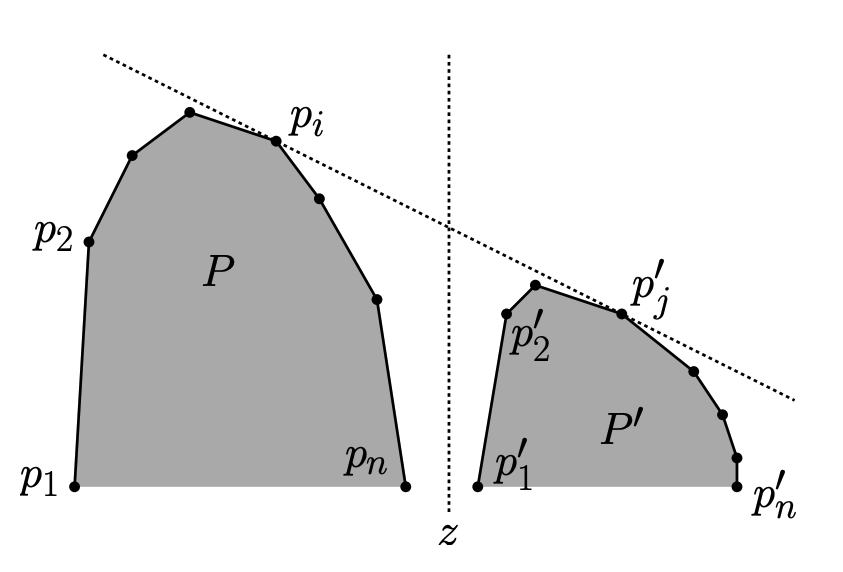
\includegraphics[width=0.5\textwidth]{tangents}
%    \caption{Problem 1: Computing the upper tangent of two hulls}
%\end{figure}

Present an $O(\log n)$-time algorithm which, given $P$ and $P'$, compute the two
points $p_i \in P$ and $p_j' \in P'$ such that their common support line passes
through these two points.

Briefly justify your algorithm's correctness and derive its running time.  ({\bf
Hint:} The correctness proof involves a case analysis.  Please be careful, a
poorly drawn figure may lead to an incorrect hypothesis.) \\

\answer


\newpage
\section*{Problem 2}

Consider a set $P = \{p_1, \ldots, p_n \}$ of points in the plane, where $p_i =
(x_i, y_i)$. A \emph{Pareto set} for $P$, denoted $\pareto{P}$, (named after
the Italian engineer and economist Vilfredo Pareto), is the smallest subset of points
such that for all $p_i \in P$ there exists a $p_j \in \pareto{P}$ such that $x_i \leq x_j$ and
$y_i \leq y_j$.

%\begin{figure}[h]
%    \centering
%    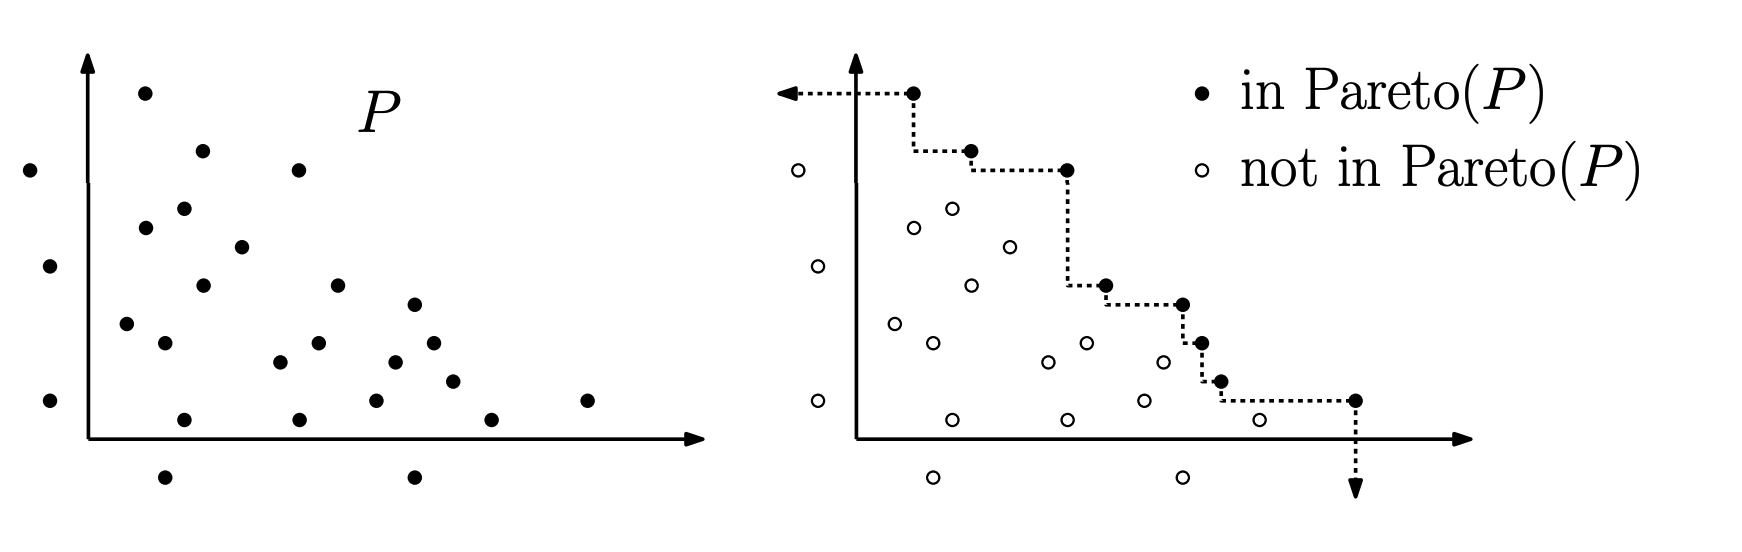
\includegraphics[width=0.75\textwidth]{pareto}
%    \caption{Problem 2: Pareto set}
%\end{figure}

Pareto sets and convex hulls in the plane are similar in many respects.  In
this problem we will explore some of these connections.

\begin{enumerate}

\item A point $p$ lies on the convex hull of a set $P$ if and only if there is
a line passing though $p$ such that all the points of $P$ lie on one side of
this line.  Provide an analogous assertion for the points of $\pareto{P}$ in
terms of a different shape.

\item Devise an analogue of Graham's convex-hull algorithm for computing
\pareto{P} in $O(n \log n)$ time.  Briefly justify your algorithm's correctness
and derive its running time.  (You do not need to explain the algorithm ``from
scratch'', that is, you can explain with modifications would be made to Grahm's
algorithm.)

\item Devise an analogue of the Jarvis march algorithm for computing
$\pareto{P}$ in $O(h \cdot n)$ time, where $h$ is the cardinality of
$\pareto{P}$.  (As with the previous part, you can just explain the differences
with Jarvis's algorithm.)

\item Devise an algorithm for computing $\pareto{P}$ in $O(n
\log h)$ time, where $h$ is the cardinality of $\pareto{P}$.

\end{enumerate}

\answer
\begin{enumerate}
    \item Our goal is to provide some geometric condition that conveys whether a point is a member of $\pareto{P}$.
    For the convex hull, a point $p$ was on the convex hull of a set $P$ if and only if there is a line passing through $p$ such that all points of $P$ lie on one side of the line.
    This is equivalent to requiring that there exists a half plane (with $p$ on the line defining the half plane) such that all points in $P$ are on one side of the half plane.
    For the $\pareto{P}$, we have a similar requirement with a ``quarter'' plane.
    Consider a plane with $p$ at the origin and axes in the regular directions.
    Then $p$ is in $\pareto{P}$ if and only if no points in $P$ are inside (or on the border) of the first quadrant of the plane centered at $p$.
    If $p$ is in the $\pareto{P}$ then no point $p'$ has both $x' \geq x$ and $y' \geq y$ so no values can be in the first quadrant.
    Proving the converse (via contrapositive), if some point $p'$ is inside the first quadrant, then both $x' \geq x$ and $y' \geq y$ so $p$ cannot be in $\pareto{P}$.

    \item First we give a quick description of the algorithm (relative to Graham's Scan).
    Instead of sorting the points in increasing order (like Graham's Scan), sort them in decreasing order according to their $x$ coordinate: $P = \{ p_1, p_2, ..., p_n \}$ where $i < j$ implies $x_i > x_j$.
    Then push $p_1$ on to the stack $S$.
    Then for $i$ from $2$ to $n$, if $y_i \geq S[top]_y$ (where $S[top]_y$ is the $y$ coordinate of the point $S[top]$) then push $p_i$ to the stack.
    We give the pseudocode below.

    \begin{algorithm}
    \caption{Computing $\pareto{P}$}
    \label{alg:paretoscan}
        \begin{algorithmic}[1]
        \Function{ParetoScan}{$P$}
            \State sort $P$ in decreasing order according the x coordinates
            \State push $p_1$ on to stack S
            \For{$i \gets 2, 3, ..., n$}
                \If{$y_i \geq S[top]_y$}
                    \State push $p_i$ on the $S$
                \EndIf
            \EndFor
            \State \Return $S$
        \EndFunction
        \end{algorithmic}
    \end{algorithm}

    Now let's analyze the runtime.
    The sorting step takes $O(n \log n)$ time and then we do a scan through all the data points in $O(n)$ time.
    So the total run time for this algorithm is $O(n \log n) + O(n) = O(n \log (n) + n) = O(n \log n)$.

    Now we give a discussion of correctnes.
    Post sorting, we know $p_1 \in \pareto{P}$ by the following line of reasoning.
    The definition of $\pareto{P}$ is the smallest subset of points such that for all $p_i \in P$ there exists a $p_j \in \pareto{P}$ such that $x_i \leq x_j$ and $y_i \leq y_j$.
    The point $p_1$ is the point with the largest $x$ coordinate, so if $p_1 \notin \pareto{P}$ then there would be no point in $\pareto{P}$ with a larger $x$ coordinate.
    Similarly, the point with the largest $y$ coordinate is also in $\pareto{P}$; we will use this fact in the next paragraph.

    Now let $P_i = \{ p_1, p_2, ..., p_i \}$.
    We claim that after attempting to insert $p_i$ to $S_i$ (the stack at iteration $i$), the stack $S_i$ contains $\pareto{P_i}$ and $S[top]$ has the largest $y$ coordinate in $P_i$.
    Consider the base case $P_1 = \{ p_1 \}$ then $\pareto{P_1} = \{ p_1 \}$ which matches $S_1$ since $p_1$ is inserted at the beginning and $S_1[top]$ has the largest $y$ coordinate since there is only one point.
    Now suppose that we have $S_i = \pareto{P_i}$ where $i \in \{ 1, 2, ..., n-1 \}$ and $S_i [top]$ has the largest $y$ coordinate in $P_i$.
    We attempt to prove that $S_{i+1}$ contains $\pareto{P_{i+1}}$.
    Since $P_{i+1} = P_i \cup \{ p_{i+1} \} $ and $S_{i+1}$ at least contains $\pareto{P_i}$ we need only check $p_{i+1}$.
    We already know $p_{i+1}$ is the furthest left point we have considered.
    So, if $y_{i+1} < S[top]_y$ then $S[top]$ is a point that prevents $p_{i+1}$ from being in $\pareto{P_{i+1}}$.
    If $y_{i+1} \geq S[top]_y$ then $p_{i+1}$ has the largest $y$ coordinate so $p_{i+1} \in \pareto{P}$.
    The algorithm matches these actions by inserting or not inserting $p_{i+1}$ into $S_{i+1}$.
    Then when the algorithm terminates we have $\pareto{P}$.

    \item Now we give an algorithm similar to the Jarvis march that computes $\pareto{P}$ in $O(h \cdot n)$ time.
    For this algorithm, we only need to find $h$ points that we know to be in $\pareto{P}$.
    First we scan through the data set to find the point $p$ with the right-most x coordinate.
    Then let $p_k$ be the last point added to the pareto.
    We scan throught the data set to find the point right most point $p_i$ such that $y_i \geq y_k$.
    We then repeat the previous step $h-1$ times (since we already have one point from step 1).
    We give the pseudocode below.

    \begin{algorithm}
    \caption{Computing $\pareto{P}$}
    \label{alg:paretostairs}
        \begin{algorithmic}[1]
        \Function{ParetoStairs}{$P, h$}
            \State scan $P$ to find right most point $p_1$
            \State push $p_1$ on to stack S
            \For{$i \gets 2, 3, ..., h$}
                \State scan $P$ to find the furthest right $p_j$ such that $y_j \geq S[top]_x$
                \State push $p_j$ to $S$
            \EndFor
            \State \Return $S$
        \EndFunction
        \end{algorithmic}
    \end{algorithm}

    As far as run time goes, the algorithm performs $h$ scans of a data set with size $n$ so the run time is $O(h \cdot n)$.
    Now for correctness, we assume that $|\pareto{P}| = h$ so we need only find $h$ points that must be part of $\pareto{P}$.
    To show correctness, we will just show that each point added must be the next point in $\pareto{P}$ (sorted in decreasing x coordinates).
    The first point added (the right most) is certainly in $\pareto{P}$, as discussed before.
    Now suppose that we have the first $i$ points of the $\pareto{P}$ in decreasing order (the partial pareto).
    We show that the next point added to the partial is the $i+1$ point in $\pareto{P}$.
    The next point $p_{i+1}$ we add is the furthest right point in the data set that is above the $p_i$ point (the $i^{th}$ point in the partial).
    Suppose there were some point $p'$ in the final pareto in between $p_{i+1}$ and $p_i$.
    Then we must have $x_{i+1} \leq x' \leq x_i$ and $y' \geq y_i$.
    But this is a contradiction since $p_{i+1}$ is the furthest right point with a y coordinate larger than $y_i$ so $p_{i+1}$ is the next point in the final pareto.
    Thus, the output of the algorithm is $\pareto{P}$.

    \item We must give an algorithm that computes $\pareto{P}$ in $O(n \log h)$ time where $|\pareto{P}| = h$.
    In prose, we will break the initial set $P$ down into $n/h$ subsets of maximum size $h$.
    Then we can find the pareto for each subset using Algorithm \ref{alg:paretostairs}.
    Finally, we merge the mini paretos into one final pareto.
    The merging process is somewhat similar to mergesort.
    For each mini pareto $A_k$, we have an index $i$ pointing to an element $A_k[i]$ that increments to $i+1$ when we merge the element $A_k[i]$.

    \begin{algorithm}
    \caption{Computing $\pareto{P}$}
    \label{alg:paretochan}
        \begin{algorithmic}[1]
        \Function{ParetoChan}{$P, h$}
            \State break $P$ into $P_1, P_2, ..., P_{n/h}$ such that $|P_i| \leq h$
            \State compute $\pareto{P_i}$ using Algorithm \ref{alg:paretostairs}, storing each pareto in an array $A_k$
            \State find $p_1$, the furthest right point of any $A_k[0]$
            \State push $p_1$ to stack $S$
            \For{$i \gets 2, 3, ..., h$}
                \State find $p_j$ the furthest right element in any $A_k$ such that $y_j \geq S[top]_y$
                \State push $p_j$ to $S$
            \EndFor
            \State \Return $S$
        \EndFunction
        \end{algorithmic}
    \end{algorithm}

    We claim the runtime of this algorithm is $O(n \log h)$.
    Breaking up the subsets takes $O(n)$ time and then computing the pareto of each subset takes $O(h \log h)$.
    Since there are $n/h$ subsets the entire mini pareto process takes $O(n \log h)$ time.
    So we are on the right track, as long as we merge quickly enough.
    Selecting an element to merge takes $O(n/h)$ time since there are $n/h$ mini paretos and we consider one element from each mini pareto.
    But we must select an element $h$ times so the total merge time is $O(n)$.
    Therefore, the algorithm runs in $O(n \log h)$ time.

    For correctness, we already know that Algorithm \ref{alg:paretostairs} is correct so we need only show that the merging is correct.
    The merging process is similar to proving that Algorithm \ref{alg:paretostairs}'s scan finds the next point in the pareto so we defer to the correctness to that proof.
    %The only thing we need to show is the existence of the next point in the subset that we are considering (recall that we only consider one element from each mini pareto at a time while merging).
    %To prove this, we only have to remember that each array $A_k$ is also a pareto (sorted by decreasing x coordinates). --- not sure if this is necessary

\end{enumerate}

\newpage
\section*{Problem 3}

Assume you have an orientation test available which can determine in constant
time whether three points make a left turn (i.e., the third point lies on the
left of the oriented line described by the first two points) or a right turn.
Now, let a point $q$ and a convex polygon $P = \{ p_1, \ldots , p_n \}$ in the
plane be given, where the points of $P$ are stored in an array in
counter-clockwise order around $P$ and $q$ is outside of $P$. Give pseudo-code
to determine the tangents from $q$ to $P$ in $O(\log n)$ time. \\

\answer
We begin by establishing a lemma about tanget lines in the context of this problem: the line $\overline{qp_k}$ is tangent to $P$ if and only if $sgn(orient(q, p_{k+1}, p_k)) \neq sgn(orient(q, p_k, p_{k-1}))$.
Going to the right, suppose that the line $\overline{qp_k}$ is tangent to $P$.
Then the points $p_{k-1}, p_{k+1}$ must be on the same side of $\overline{q p_k}$.
Then (hopefully) Figure \ref{fig:tangent} is convincing evidence to say that $sgn(orient(q, p_{k+1}, p_k)) \neq sgn(orient(q, p_k, p_{k-1}))$.

\begin{figure}[h]
    \centering
    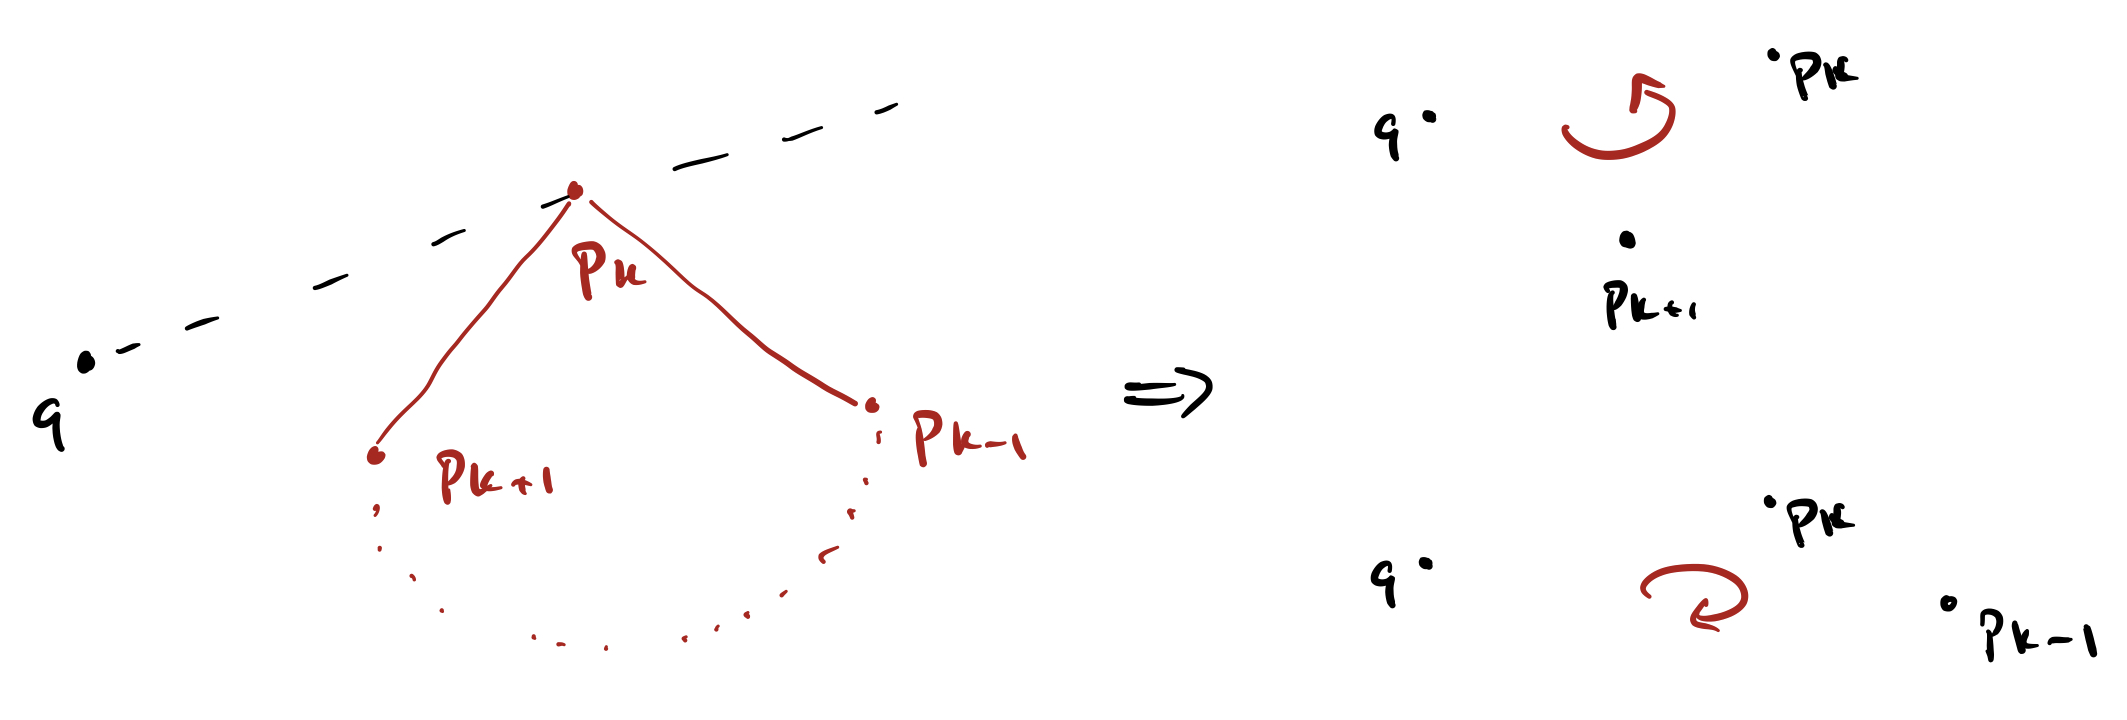
\includegraphics[width=0.75\textwidth]{tangent}
    \caption{Line $\overline{q p_k}$ is tangent to $P$}
    \label{fig:tangent}
\end{figure}

Now going to the left, we will show the contrapositive.
Suppose that $sgn(orient(q, p_{k+1}, p_k)) = sgn(orient(q, p_k, p_{k-1}))$.
Here we can say that $p_{k-1}$ and $p_{k+1}$ must lie on opposite sides of the line $\overline{q p_k}$ (Figure \ref{fig:nottangent} depicts an example).
But then $\overline{q p_k}$ cannot be a tangent line so the contrapositive is shown.

\begin{figure}[h]
    \centering
    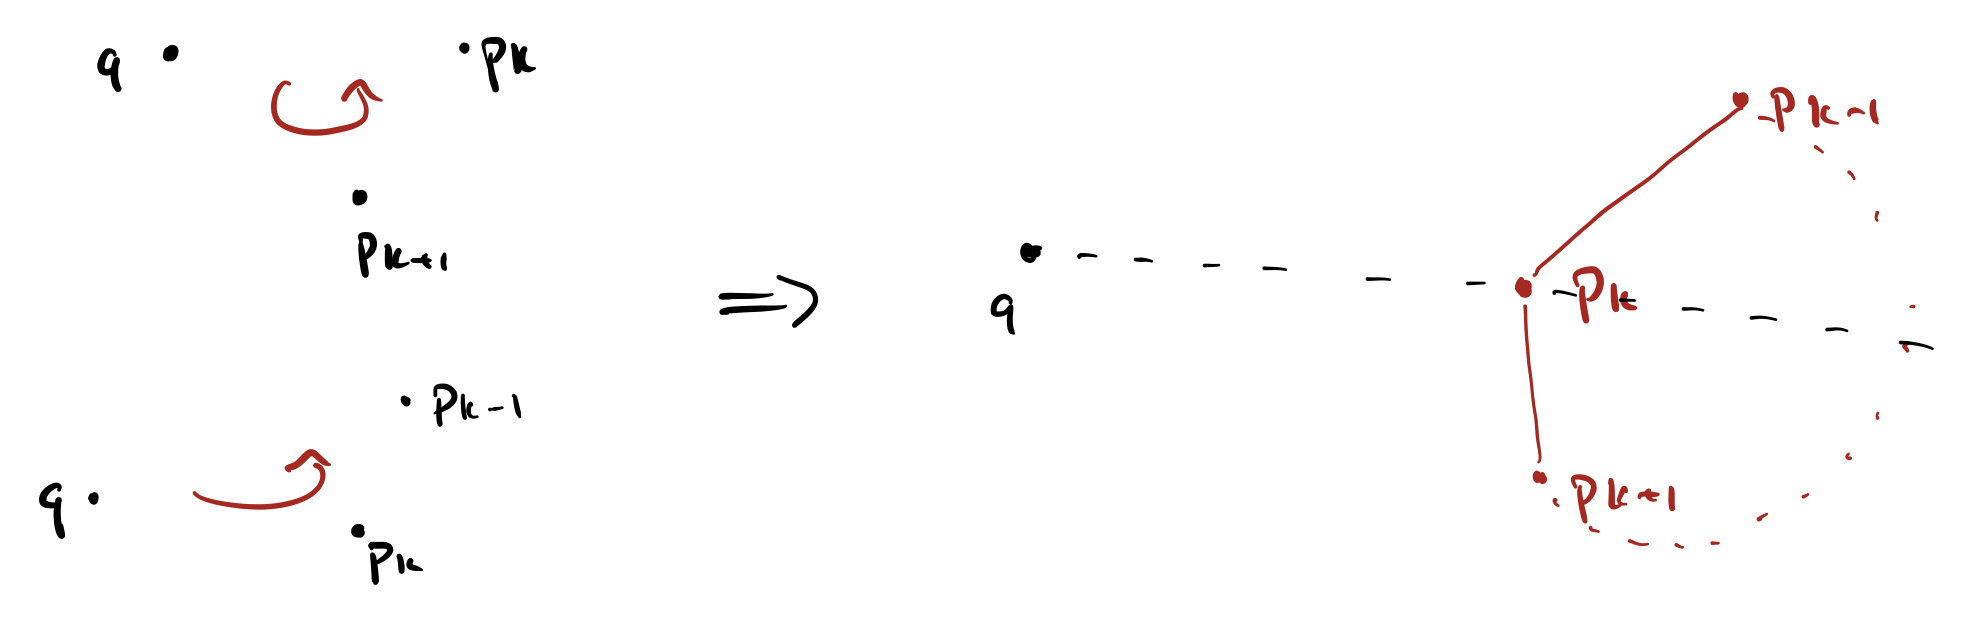
\includegraphics[width=0.75\textwidth]{nottangent}
    \caption{Line $\overline{q p_k}$ is not tangent to $P$}
    \label{fig:nottangent}
\end{figure}

Now we can use the lemma to construct an $O(\log n)$ algorithm to find the tangent lines from $q$ to $P$.

\begin{algorithm}
    \caption{Compute tangent lines from $q$ to $P$}
    \begin{algorithmic}
        \State $y \gets 1$
    \end{algorithmic}
\end{algorithm}

\newpage
\section*{Problem 4}

Given a set $S$ of $n$ points in the plane, consider the subsets

\begin{eqnarray*}
	S_1 &=& S, \\
	S_2 &=& S_1 \setminus \{ \text{set of vertices of } \conv{S_1} \} \\
		&\ldots& \\
	S_i &=& S_{i-1} \setminus \{ \text{set of vertices of } \conv{S_{i-1}} \}
\end{eqnarray*}
%
until $S_k$ has at most three elements.  Give an $O(n^2)$ time algorithm that
computes all convex hull $\conv{S_1}, \conv{S_2}, \ldots, S_k$.  [Extra credit,
provide an algorithm that is faster than $O(n^2)$]. \\

%\begin{figure}[h]
%    \centering
%    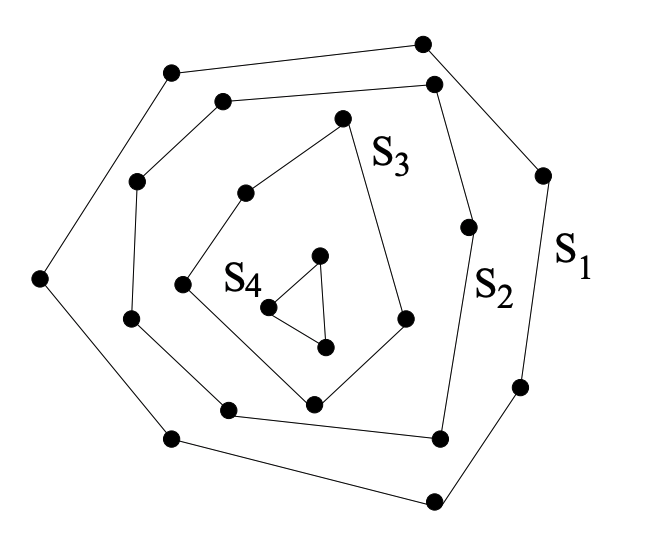
\includegraphics[width=0.25\textwidth]{onions}
%    \caption{Problem 4: Onion peeling}
%\end{figure}

\answer
To find all $\conv{S_i}$ in $O(n^2)$ time, we use a modified version of Graham's Scan.
In words, we run Graham's Scan on $S$ but keep track of a stack for each $\conv{S_i}$.
When we pop a set of points off the stack $T_k$ we move the set down to the next stack and repeat Graham's Scan for the stack $T_{k+1}$.
Here is the pseudocode.

\begin{algorithm}
\caption{Computing the onion}
    \label{alg:onion}
    \begin{algorithmic}[1]
    \Function{ComputeOnion}{$S$}
        \State sort points in increasing order according to $x$
        \State push $p_1, p_2$ on to the first stack $T_1$
        \For{$i \gets 3, 4, ..., n$}
            \State $T \gets T_1$
            \State $popped \gets Pop(A=[p_i], T)$
            \While{$popped$ is not empty}
                \State $T \gets$ the next stack
                \State $popped \gets Pop(popped, S)$
            \EndWhile
        \EndFor
        \State \Return $T_1, T_2, ..., T_k$
    \EndFunction
    \end{algorithmic}

    \begin{algorithmic}[1]
    \Function{Pop}{$A[1..k], T$}
        \State initialize popped list $L$
        \While{$|T| \geq 2$ and $Orient(A[1], T[top], T[top-1])$}
            \State append $T[top]$ to $L$ and pop $T[top]$
        \EndWhile
        \State push elements of $A$ on to $T$
        \State \Return $L.reverse()$ // reverse so elements are increasing in $x$
    \EndFunction
    \end{algorithmic}
\end{algorithm}

We claim the run time of the algorithm is $O(n^2)$.
The sorting process takes $O(n \log n)$ and we already know Graham's Scan to identify sorted points in $O(n)$ time when we only search for the outer convex hull.
The maximum number of stacks that we can have is $n/3 = O(n)$ (a bunch of concentric triangles).
In the very worst case, each Graham's Scan would take $O(n)$ time and there are $O(n)$ scans so identifying the points takes $O(n^2)$ time.

For correctness, a lot of the work is done because we are using Graham's Scan at each level.
Suppose we have a point $p$ that should end up in $\conv{S_i}$.
We begin processing the point at level $S_1$, if $i > 1$ then Graham's Scan will not keep $p$.
Thus it eventually pops $p$ and will pushes it down a level.
Since every level is using Graham's Scan, this process will repeat until $p$ encounters the stack for $\conv{S_i}$.
Since we are using Graham's Scan to find $\conv{S_i}$, $p$ will never leave the stack for $\conv{S_i}$.
Thus the algorithm is correct.

% \newpage
% \section*{Tips and Acknowledgements}
%
% {\bf David Mount's tips for writing up homework solutions}: Whenever you are
% asked to present an ``algorithm,'' you should present three things: the
% algorithm, an informal proof of its correctness, and a derivation of its
% running time.  Remember that your description is intended to be read by a
% human, not a compiler, so conciseness and clarity are preferred over technical
% details.  Unless otherwise stated, you may use any results from class, or
% results from any standard textbook on algorithms and data structures. Also, you
% may use results from geometry that: (1) have been mentioned in class, (2) would
% be known to someone who knows basic geometry or linear algebra, or (3) is
% intuitively obvious. If you are unsure, please feel free to check with me.
%
% Giving careful and rigorous proofs can be quite cumbersome in geometry, and so
% you are encouraged to use intuition and give illustrations whenever appropriate.
% Beware, however, that a poorly drawn figure can make certain erroneous
% hypotheses appear to be ``obviously correct.''
%
% Throughout the semester, unless otherwise stated, you may assume that input
% objects are in general position. For example, you may assume that no two points
% have the same x-coordinate, no three points are collinear, no four points are
% cocircular. Also, unless otherwise stated, you may assume that any geometric
% primitive involving a constant number of objects each of constant complexity can
% be computed in O(1) time
%
% {\bf Acknowledgements:} Homework problems adapted from assignments of David
% Mount and Carola Wenk.

\end{document}
